%  A simple AAU report template.
%  2015-05-08 v. 1.2.0
%  Copyright 2010-2015 by Jesper Kjær Nielsen <jkn@es.aau.dk>
%
%  This is free software: you can redistribute it and/or modify
%  it under the terms of the GNU General Public License as published by
%  the Free Software Foundation, either version 3 of the License, or
%  (at your option) any later version.
%
%  This is distributed in the hope that it will be useful,
%  but WITHOUT ANY WARRANTY; without even the implied warranty of
%  MERCHANTABILITY or FITNESS FOR A PARTICULAR PURPOSE.  See the
%  GNU General Public License for more details.
%
%  You can find the GNU General Public License at <http://www.gnu.org/licenses/>.
%
%  A simple AAU report template.
%  2015-05-08 v. 1.2.0
%  Copyright 2010-2015 by Jesper Kjær Nielsen <jkn@es.aau.dk>
%
%  This is free software: you can redistribute it and/or modify
%  it under the terms of the GNU General Public License as published by
%  the Free Software Foundation, either version 3 of the License, or
%  (at your option) any later version.
%
%  This is distributed in the hope that it will be useful,
%  but WITHOUT ANY WARRANTY; without even the implied warranty of
%  MERCHANTABILITY or FITNESS FOR A PARTICULAR PURPOSE.  See the
%  GNU General Public License for more details.
%
%  You can find the GNU General Public License at <http://www.gnu.org/licenses/>.
%
\documentclass[11pt,twoside,a4paper,openright]{report}
%%%%%%%%%%%%%%%%%%%%%%%%%%%%%%%%%%%%%%%%%%%%%%%%
% Language, Encoding and Fonts
% http://en.wikibooks.org/wiki/LaTeX/Internationalization
%%%%%%%%%%%%%%%%%%%%%%%%%%%%%%%%%%%%%%%%%%%%%%%%
% Select encoding of your inputs. Depends on
% your operating system and its default input
% encoding. Typically, you should use
%   Linux  : utf8 (most modern Linux distributions)
%            latin1 
%   Windows: ansinew
%            latin1 (works in most cases)
%   Mac    : applemac
% Notice that you can manually change the input
% encoding of your files by selecting "save as"
% an select the desired input encoding. 
\usepackage[utf8]{inputenc}
% Make latex understand and use the typographic
% rules of the language used in the document.
\usepackage[danish,english]{babel}
% Use the palatino font
\usepackage[sc]{mathpazo}
\linespread{1.05}         % Palatino needs more leading (space between lines)
% Choose the font encoding
\usepackage[T1]{fontenc}
%%%%%%%%%%%%%%%%%%%%%%%%%%%%%%%%%%%%%%%%%%%%%%%%
% Graphics and Tables
% http://en.wikibooks.org/wiki/LaTeX/Importing_Graphics
% http://en.wikibooks.org/wiki/LaTeX/Tables
% http://en.wikibooks.org/wiki/LaTeX/Colors
%%%%%%%%%%%%%%%%%%%%%%%%%%%%%%%%%%%%%%%%%%%%%%%%
% load a colour package
\usepackage{xcolor}
\definecolor{aaublue}{RGB}{33,26,82}% dark blue
% The standard graphics inclusion package
\usepackage{graphicx}
% Set up how figure and table captions are displayed
\usepackage{float}
% Allow placement of figure with the H option
\usepackage{caption}
\captionsetup{%
  font=footnotesize,% set font size to footnotesize
  labelfont=bf % bold label (e.g., Figure 3.2) font
}
% Make the standard latex tables look so much better
\usepackage{array,booktabs}
% Enable the use of frames around, e.g., theorems
% The framed package is used in the example environment
\usepackage{framed}

%%%%%%%%%%%%%%%%%%%%%%%%%%%%%%%%%%%%%%%%%%%%%%%%
% Mathematics
% http://en.wikibooks.org/wiki/LaTeX/Mathematics
%%%%%%%%%%%%%%%%%%%%%%%%%%%%%%%%%%%%%%%%%%%%%%%%
% Defines new environments such as equation,
% align and split 
\usepackage{amsmath}
% Adds new math symbols
\usepackage{amssymb}
% Use theorems in your document
% The ntheorem package is also used for the example environment
% When using thmmarks, amsmath must be an option as well. Otherwise \eqref doesn't work anymore.
\usepackage[framed,amsmath,thmmarks]{ntheorem}

%%%%%%%%%%%%%%%%%%%%%%%%%%%%%%%%%%%%%%%%%%%%%%%%
% Page Layout
% http://en.wikibooks.org/wiki/LaTeX/Page_Layout
%%%%%%%%%%%%%%%%%%%%%%%%%%%%%%%%%%%%%%%%%%%%%%%%
% Change margins, papersize, etc of the document
\usepackage[
    left=28mm,% left margin on an odd page
    right=28mm,% right margin on an odd page
    top=28mm,
    bottom=28mm
 ]{geometry}
% Modify how \chapter, \section, etc. look
% The titlesec package is very configureable
\usepackage{titlesec}
\titleformat{\chapter}[display]{\normalfont\huge\bfseries}{\chaptertitlename\ \thechapter}{20pt}{\Huge}
\titleformat*{\section}{\normalfont\Large\bfseries}
\titleformat*{\subsection}{\normalfont\large\bfseries}
\titleformat*{\subsubsection}{\normalfont\normalsize\bfseries}
%\titleformat*{\paragraph}{\normalfont\normalsize\bfseries}
%\titleformat*{\subparagraph}{\normalfont\normalsize\bfseries}

% Clear empty pages between chapters
\let\origdoublepage\cleardoublepage
\newcommand{\clearemptydoublepage}{%
  \clearpage
  {\pagestyle{empty}\origdoublepage}%
}
\let\cleardoublepage\clearemptydoublepage

% Change the headers and footers
\usepackage{fancyhdr}
\pagestyle{fancy}
\fancyhf{} %delete everything
\renewcommand{\headrulewidth}{0pt} %remove the horizontal line in the header
\fancyhead[RE]{\small\nouppercase\leftmark} %even page - chapter title
\fancyhead[LO]{\small\nouppercase\rightmark} %uneven page - section title
\fancyhead[LE,RO]{\thepage} %page number on all pages
% Do not stretch the content of a page. Instead,
% insert white space at the bottom of the page
\raggedbottom
% Enable arithmetics with length. Useful when
% typesetting the layout.
\usepackage{calc}

%%%%%%%%%%%%%%%%%%%%%%%%%%%%%%%%%%%%%%%%%%%%%%%%
% Bibliography
% http://en.wikibooks.org/wiki/LaTeX/Bibliography_Management
%%%%%%%%%%%%%%%%%%%%%%%%%%%%%%%%%%%%%%%%%%%%%%%%
%\usepackage[backend=bibtex,
%  bibencoding=utf8
%  ]{biblatex}
%\addbibresource{bib/mybib}

%%%%%%%%%%%%%%%%%%%%%%%%%%%%%%%%%%%%%%%%%%%%%%%%
% Misc
%%%%%%%%%%%%%%%%%%%%%%%%%%%%%%%%%%%%%%%%%%%%%%%%
% Add bibliography and index to the table of
% contents
%\usepackage[nottoc]{tocbibind}
% Add the command \pageref{LastPage} which refers to the
% page number of the last page
\usepackage{lastpage}
% Add todo notes in the margin of the document
% Add todo notes in the margin of the document
\usepackage[
  %disable, %turn off todonotes
  %colorinlistoftodos, %enable a coloured square in the list of todos
  textwidth=\textwidth, %set the width of the todonotes
  textsize=scriptsize, %size of the text in the todonotes
  color=blue!40!white
  ]{todonotes}
\setuptodonotes{inline}

%%%%%%%%%%%%%%%%%%%%%%%%%%%%%%%%%%%%%%%%%%%%%%%%
% Hyperlinks
% http://en.wikibooks.org/wiki/LaTeX/Hyperlinks
%%%%%%%%%%%%%%%%%%%%%%%%%%%%%%%%%%%%%%%%%%%%%%%%
% Enable hyperlinks and insert info into the pdf
% file. Hypperref should be loaded as one of the 
% last packages
\usepackage{hyperref}
\hypersetup{%
	pdfpagelabels=true,%
	plainpages=false,%
	pdfauthor={Author(s)},%
	pdftitle={Title},%
	pdfsubject={Subject},%
	bookmarksnumbered=true,%
	colorlinks=false,%
	citecolor=black,%
	filecolor=black,%
	linkcolor=black,% you should probably change this to black before printing
	urlcolor=black,%
	pdfstartview=FitH%
}

\usepackage{stuffbyanders}% package inclusion and set up of the document
% see, e.g., http://en.wikibooks.org/wiki/LaTeX/Formatting#Hyphenation
% for more information on word hyphenation
\hyphenation{ex-am-ple hy-phen-a-tion short}
\hyphenation{long la-tex}% 
%  A simple AAU report template.
%  2015-05-08 v. 1.2.0
%  Copyright 2010-2015 by Jesper Kjær Nielsen <jkn@es.aau.dk>
%
%  This is free software: you can redistribute it and/or modify
%  it under the terms of the GNU General Public License as published by
%  the Free Software Foundation, either version 3 of the License, or
%  (at your option) any later version.
%
%  This is distributed in the hope that it will be useful,
%  but WITHOUT ANY WARRANTY; without even the implied warranty of
%  MERCHANTABILITY or FITNESS FOR A PARTICULAR PURPOSE.  See the
%  GNU General Public License for more details.
%
%  You can find the GNU General Public License at <http://www.gnu.org/licenses/>.
%
%
%
% see, e.g., http://en.wikibooks.org/wiki/LaTeX/Customizing_LaTeX#New_commands
% for more information on how to create macros

%%%%%%%%%%%%%%%%%%%%%%%%%%%%%%%%%%%%%%%%%%%%%%%%
% Macros for the titlepage
%%%%%%%%%%%%%%%%%%%%%%%%%%%%%%%%%%%%%%%%%%%%%%%%
%Creates the aau titlepage
\newcommand{\aautitlepage}[3]{%
  {
    %set up various length
    \ifx\titlepageleftcolumnwidth\undefined
      \newlength{\titlepageleftcolumnwidth}
      \newlength{\titlepagerightcolumnwidth}
    \fi
    \setlength{\titlepageleftcolumnwidth}{0.5\textwidth-\tabcolsep}
    \setlength{\titlepagerightcolumnwidth}{\textwidth-2\tabcolsep-\titlepageleftcolumnwidth}
    %create title page
    \thispagestyle{empty}
    \noindent%
    \begin{tabular}{@{}ll@{}}
      \parbox{\titlepageleftcolumnwidth}{
        \iflanguage{danish}{%
          
\includegraphics[width=\titlepageleftcolumnwidth]{figures/aau_logo_da}
        }{%
          
\includegraphics[width=\titlepageleftcolumnwidth]{figures/aau_logo_en}
        }
      } &
      \parbox{\titlepagerightcolumnwidth}{\raggedleft\sf\small
        #2
      }\bigskip\\
       #1 &
      \parbox[t]{\titlepagerightcolumnwidth}{%
      \textbf{Abstract:}\bigskip\par
        \fbox{\parbox{\titlepagerightcolumnwidth-2\fboxsep-2\fboxrule}{%
          #3
        }}
      }\\
    \end{tabular}
    \vfill
    \iflanguage{danish}{%
      \noindent{\footnotesize\emph{Rapportens indhold er frit tilgængeligt, men offentliggørelse (med kildeangivelse) må kun ske efter aftale med forfatterne.}}
    }{%
      \noindent{\footnotesize\emph{The content of this report is freely available, but publication (with reference) may only be pursued due to agreement with the author.}}
    }
    \clearpage
  }
}

%Create english project info
\newcommand{\englishprojectinfo}[8]{%
  \parbox[t]{\titlepageleftcolumnwidth}{
    \textbf{Title:}\\ #1\bigskip\par
    \textbf{Theme:}\\ #2\bigskip\par
    \textbf{Project Period:}\\ #3\bigskip\par
    \textbf{Project Group:}\\ #4\bigskip\par
    \textbf{Participant(s):}\\ #5\bigskip\par
    \textbf{Supervisor(s):}\\ #6\bigskip\par
    \textbf{Copies:} #7\bigskip\par
    \textbf{Page Numbers:} \pageref{LastPage}\bigskip\par
    \textbf{Date of Completion:}\\ #8
  }
}

%Create danish project info
\newcommand{\danishprojectinfo}[8]{%
  \parbox[t]{\titlepageleftcolumnwidth}{
    \textbf{Titel:}\\ #1\bigskip\par
    \textbf{Tema:}\\ #2\bigskip\par
    \textbf{Projektperiode:}\\ #3\bigskip\par
    \textbf{Projektgruppe:}\\ #4\bigskip\par
    \textbf{Deltager(e):}\\ #5\bigskip\par
    \textbf{Vejleder(e):}\\ #6\bigskip\par
    \textbf{Oplagstal:} #7\bigskip\par
    \textbf{Sidetal:} \pageref{LastPage}\bigskip\par
    \textbf{Afleveringsdato:}\\ #8
  }
}

%%%%%%%%%%%%%%%%%%%%%%%%%%%%%%%%%%%%%%%%%%%%%%%%
% An example environment
%%%%%%%%%%%%%%%%%%%%%%%%%%%%%%%%%%%%%%%%%%%%%%%%
\theoremheaderfont{\normalfont\bfseries}
\theorembodyfont{\normalfont}
\theoremstyle{break}
\def\theoremframecommand{{\color{gray!50}\vrule width 5pt \hspace{5pt}}}
\newshadedtheorem{exa}{Example}[chapter]
\newenvironment{example}[1]{%
		\begin{exa}[#1]
}{%
		\end{exa}
}% my new macros

\graphicspath{{figures/}}


\begin{document}
%frontmatter
\pagestyle{empty} %disable headers and footers
\pagenumbering{roman} %use roman page numbering in the frontmatter
\cleardoublepage
\pdfbookmark[0]{Contents}{label:contents}
\pagestyle{fancy} %enable headers and footers again
\tableofcontents
\listoftodos
%\input{sections/preface.tex}
\cleardoublepage
%mainmatter
\pagenumbering{arabic} %use arabic page numbering in the mainmatter


%%%%%% SECTIONS


\chapter{Introduction}\label{ch:introduction}

The case chosen for this assignment was project 3 regarding simulator for wireless communication. Based on the assignment description, the report will contain information about all the phases of the project; Analysis, Design, how the design was implemented, major decisions that we needed to take and finally the live product.\newline

The wireless network simulator involved designing a software that simulates wireless communication between nodes. Furthermore, the nodes are to be places in different position in a user defined space and they are to communicate with each other. In the assignment description, the program is required to have these additional aspects:
\begin{itemize}
    \item User must choose different type of nodes such as base stations, mobile phones, drones, satellites...
    \item A subset of nodes may transmit a block of data selecting a certain power, frequency, bandwidth and time of transmission
    \item A subset of nodes may listen to incoming data and try to decode the data
    \item A GUI is used to insert and remove nodes. It is also used to start and stop data communication and to show communication quality information of each node 
\end{itemize}

We then proceeded to carry on with the first stage of the waterfall model which is Analysis. During the Analysis, we discovered additional considerations that we would need to take into account. This resulted in the group coming up with a use-case diagram and a class diagram. Then the simulator was implemented in python. During this project, the group had encountered some challenges which would be discussed in the report.








\chapter{Analysis}\label{ch:Analysis}

In the first step of the waterfall model, requirement and object analysis is carried out.

\section{Defining use cases}
Based on the description given, actors and use cases are identified and then clearly defined.

\subsection{Actors}
Based on the project description provided, the only actor that we have found would be the user who is running the simulation. At first we had considered the database to be an actor of the system but later discovered that it would not be that appropriate to have the database as an actor to the system.

\subsection{Use cases}
Next, we have defined the various use cases that we want the user to be able to do, which will be described in the following sections.

\subsubsection{Add node}
When the user wants to add the node, they would need to specify the type of node added. The node added could be either a IoT Node or a network gateway.

\subsubsection{Start Simulation}
When the user wants to start the simulation, they would need to provide the following information:
\begin{itemize}
  \item Number of nodes in the network
  \item Size of the 2D grid where the nodes will be placed
  \item Option of verbose output
\end{itemize}

\subsubsection{See simulation statistics}
When the user wants to see simulation statistics, the system would need to check if any simulation has occurred previously. If there is no prior simulation, then the system would display an error. Otherwise, the system would display the simulation statistics such as throughput, delay, and packet loss.

\subsection{Use case diagram}
Based on the factors mentioned above, a use case diagram was developed. The use case diagram can be seen below.

\subsection{FURPS}

The FURPS were utilized to better define the system's requirements. The system's overall summary was also created using this technique. This approach also aided in providing a fresh and more enlightening perspective on the issue and the requirements.

\subsubsection{Functionality: what should the system do?}
\begin{itemize}
  \item The system should be able to place the nodes in a grid and transmit packets from one node to the gateway.

        %\item The system would need to place different type of nodes in the network

  \item The system would need to run the simulation for a fixed amount of time


\end{itemize}

\subsubsection{Usability: what kind of UI is needed?}
\begin{itemize}
  \item A screen would be required to display the simulation statistics
  \item A device should receive user input eg.keyboard
\end{itemize}

\subsubsection{Reliability: what is the tolerance of the system to failures?}
\begin{itemize}
  \item The system should be able to check if the simulation has been run before displaying simulation statistics
\end{itemize}

\subsubsection{Performance: which response times, accuracy, availability, resource usage should the system have?}

\begin{itemize}
  \item The GUI needs to be run on a simple computer
  \item The simulation statistics needs to be stored in a server
\end{itemize}

\subsubsection{Sustainability: what adaptations may be needed?}
\begin{itemize}
  \item The system need to give the user the ability to change the simulation conditions after a run has been completed
\end{itemize}

\section{Domain model}
To aid the group in identifying the various objects involved in the problem, a domain model was developed. Firstly, the identified actor, which is the user, is represented as a GUI in the model. This also constitutes the front end of the system. Regarding the back end of the system, we would need one object to simulate the network and another one to generate/store the simulation statistics. Ultimately, we would need an object for the devices themselves and one for the overall network. Here it might also be a viable option to differentiate between a node object and a gateway object that then both can inherit attributes and methods from the device object when making the class diagram. Then, in order to control everything and tie the simulation to gather, it would make sense to incorporate a simulation object that handles the simulation itself.

\begin{figure}[H]
  \centering
  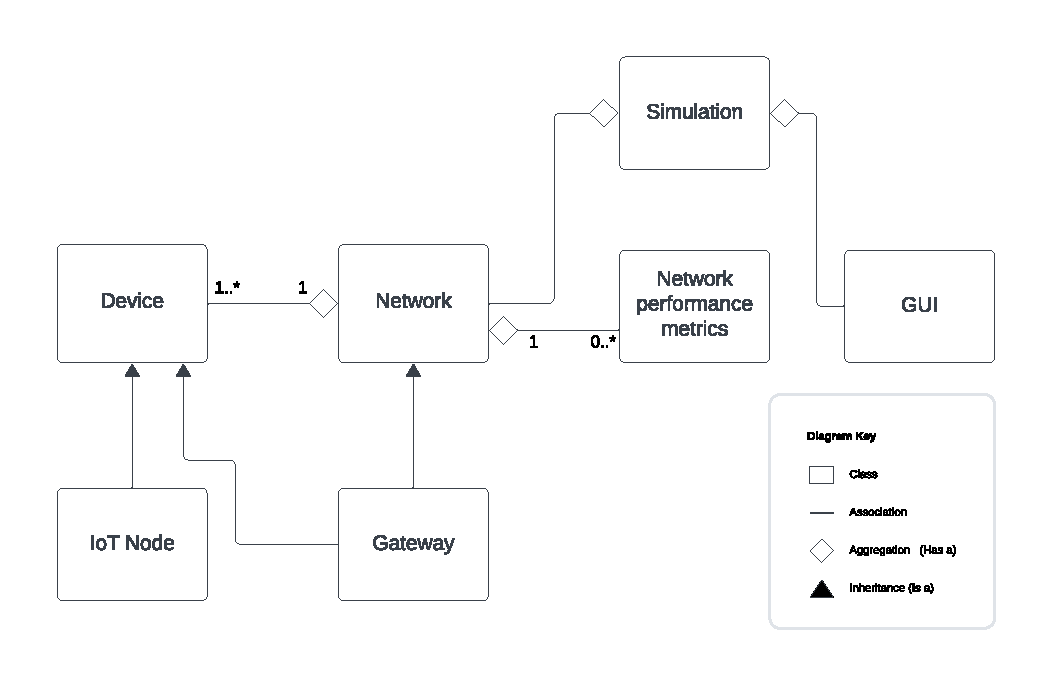
\includegraphics[width=\textwidth]{Domain_model.pdf}
  \caption{Diagram of the domain model.}
  \label{fig:Domain_model}
\end{figure}

\section{Class diagram}
The entirety of the class diagram can be seen in \autoref{fig:Class_diagram}. The parts that were not implemented have their text colored red. This also implies that the class diagram is made in accordance to how the implementation has been done, where it then has been changed whenever something has been changed in the program itself.

\begin{figure}[H]
  \centering
  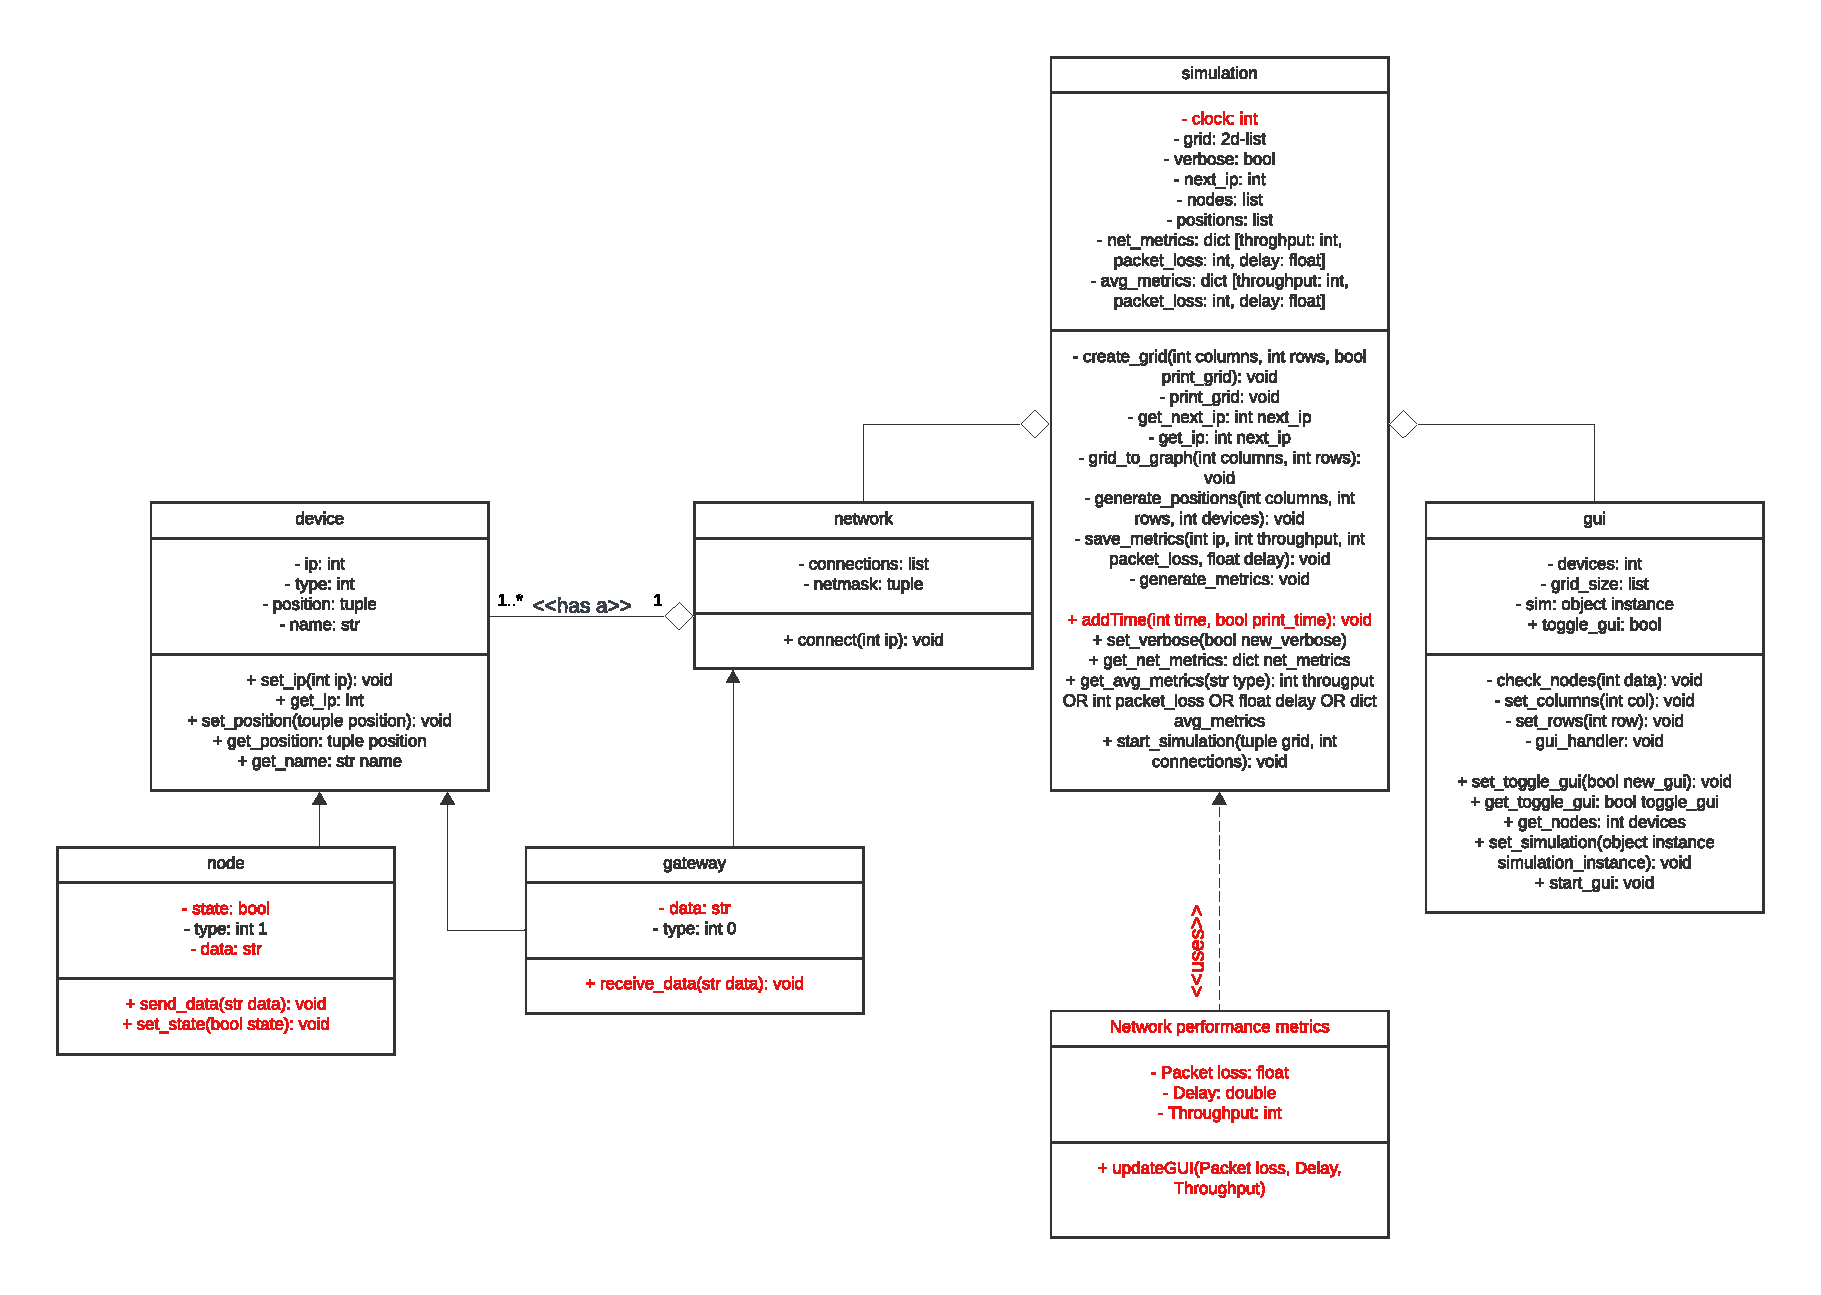
\includegraphics[width=\textwidth]{UML class diagram.pdf}
  \caption{Diagram of the classes.}
  \label{fig:Class_diagram}
\end{figure}

\subsection{GUI} It needs to be possible for the rest of the system to function without a GUI, which will also make it easier to test whether the rest of the program functions as expected. Since this is also the object that the user will interact with, it should also be somewhat easy to use. In order to start the GUI itself a \code{start\_gui} method is needed that can then be called from the main program file. Since PyWebIO is used to program the GUI, the built-in method, called \code{start\_server} can then be called to open a port on the transport layer, which then in turn can be used to access the GUI from any other computer with network access to the computer executing the program. When \code{start\_server} is called, another method can be passed along as an argument, which is then how the GUI is controlled for the remaining time. This method is called \code{gui\_handler}, and it decides which elements of the GUI is shown as well as receiving input from the user and calling other methods of the \code{gui} object.

\subsection{Network}
This class is missing a lot of the attributes and methods that it should have managed instead of the \code{simulation} object. As it is currently implemented, the \code{network} object only stores a list of the IP-addresses that are currently reserved by the gateway or one of the nodes.\bigbreak

\noindent Conventionally, on local networks, only the digits after the last period in the IP-addresses differentiate the different devices in the network. Therefore, it is only necessary to store the differentiating part of the IP-addresses. This means that the attribute \code{connections} must be able to contain a list of integers from 1 to some maximum number of devices in the network. Additionally, the \code{simulation} ended up being in charge of creating connections between the gateway and the nodes, even though this should definitively have been a method of the \code{device} object that \code{node} and \code{gateway} would then have been able to use to reserve an IP-address in the \code{connections} attribute of the \code{network} object.\newline

\noindent To put it differently, the \code{network} object should have more coupling to make it more clear that it is in charge of the network functionality, that its name is implying. Even though the \code{simulation} is necessary, it should have been possible to view all of the network methods and attributes in the \code{network} object instead of needing to also view the \code{simulation} object.

\subsection{Device}
As the class diagram in \autoref{fig:Class_diagram} shows, \code{device} is a superclass of \code{node} and \code{device}. This is done to avoid duplication of the methods and attributes that \code{node} and \code{gateway} share. The attribute \code{type} is set to \code{None} in the \code{device} object. This is done since this attribute is not intended to be used in an instance of the \code{device} object, since the \code{set\_ip} method takes the \code{type} and \code{ip} attributes and set the name of the device (either a \code{gateway} or \code{node}). The specific naming of devices will be further specified in \autoref{sec:Class_diagram_Node} and \autoref{sec:Class_diagram_Gateway}. In the final implementation, the \code{position} also ended up being used to store the position of a given node in itself. However, the device does not need to know its own position - only the \code{simulation} object should be aware of the position of each device since the \code{position} is only used to print the position in the terminal in the current implementation. The multiplicity between \code{network} and \code{device} is that one network can have one to many devices. However, as of the current implementation, there can only be one gateway.

\subsubsection{Node}\label{sec:Class_diagram_Node}
This subclass of the \code{device} overwrites the \code{type} attribute to 1, when an instance of it is created. The naming of each \code{node} instance is then done based on their \code{ip} attribute. The gateway uses the IP-address 1. This means that the first node has the IP-address 2. The naming of each \code{node} is therefore 'Node n', where n is 2 subtracted from the \code{ip} attribute. The attributes and methods with red text will be further touched upon in \autoref{ch:Discussion}, where the implementation will be discussed.

\subsubsection{Gateway}\label{sec:Class_diagram_Gateway}
In the final implementation, the \code{gateway} ended up being a subclass of both the \code{network} and the \code{device}. Just like the \code{node} class, the \code{gateway} overwrites the \code{type} attribute of the \code{device} class. The naming in \code{set\_ip} for a \code{gateway} with \code{type = 0} is then 'Gateway n', where n is 1 subtracted from the \code{ip} attribute, since the first and only gateway has the IP-address 1.

\subsection{Simulation}
The simulation is the object that takes over right after getting called by the \code{gui} object. It is then in charge of controlling the simulation. The first thing that happens is then that the \code{start\_simulation} method is accessed by the \code{gui\_handler} method which passes on the input from the user, namely the attributes \code{devices}, and \code{grid\_size}. By called its own method \code{simulation} can then use \code{create\_grid} to create an empty grid of the size specified by the previously mentioned attributes.\bigbreak

\noindent Right after creating the empty grid, the \code{gateway} object is instantiated, it gets the IP-address 1 by using calling the \code{get\_next\_ip} method, and its position is then set to the middle of the empty grid and stored both in the \code{gateway} object as well as the \code{simulation} object. Even though it was implemented this way it should only have been stored in the \code{gateway} object.































%%%%%%




\printbibliography[heading=bibintoc]
\label{bib:mybiblio}
%\appendix
%\input{sections/appAname.tex}
\end{document}